\chapter{Transformada de Laplace}\label{sec:laplace}
\index{transformada de Laplace}\index{Laplace, transformada de}

\section{Introducció}
La transformada de Laplace és part de l'anomenat càlcul operacional,
i s'utilitza per convertir equacions diferencials ordinàries en
equacions lineals; un cop resoltes aquestes equacions lineals, la
transformada inversa de Laplace ens proporciona la solució de
l'equació diferencial original.

\section{Definicions}\index{transformada de
Laplace!definicions}

\subsection{Transformada de Laplace}

La transformada de Laplace $\mathcal{L}$  converteix una funció del
temps $f(t)$, definida per a $t\geq 0$, en una funció $F(s)$, on $s$
és una variable complexa:
\begin{equation}
    \mathcal{L}\bigl(f(t)\bigr) \equiv F(s) = \int_0^\infty f(t) \,\eu^{-s t} \diff t =
    \lim_{\tau\to\infty} \int_0^\tau f(t) \,\eu^{-s t} \diff t \label{eq:transf_laplace}
\end{equation}

El teorema de l'existència de la transformada de Laplace estableix
que si $f(t)$ és una funció contínua a trossos en qualsevol
interval finit contingut en $[0,\infty)$, i satisfà: $|f(t)| \leq M
\eu^{\alpha t}$ per a qualsevol $t \in [0,\infty)$, llavors la
funció $\mathcal{L}\bigl(f(t)\bigr)$ existeix i és única per a
qualsevol $s > \alpha$.

\subsection{Transformada inversa de Laplace}

La transformada inversa de Laplace $\mathcal{L}^{-1}$ s'utilitza per
obtenir la funció original $f(t)$ a partir de la funció
transformada $F(s)$:
\begin{equation}
    \mathcal{L}^{-1}\bigl(F(s)\bigr) \equiv f(t) = \frac{1}{2 \piup \ju }
    \int_{\gamma-\ju \infty}^{\gamma+\ju \infty} F(s)\, \eu^{s t} \diff s
    \qquad (t\geq 0) \label{eq:transf_inv_laplace}
\end{equation}

On $\gamma$ és un camí vertical en el pla complex, escollit de tal
manera que totes les singularitats de la funció $F(s)$ quedin a la
seva esquerra.

\subsection{Funció graó unitari i funció impuls}\index{funció!graó
unitari} \index{funció!impuls}\index{funció!de
Heaviside}\index{funció!delta de Dirac}\index{Heaviside, funció
de}\index{Dirac, funció delta
de}\index{$\epsilon$@$\varepsilon_\tau(t)$}\index{$\delta_\tau(t)$}

Aquestes dues funcions són de gran importància en el càlcul
operacional. La funció graó unitari, o funció de Heaviside
$\varepsilon_\tau(t)$ o $\varepsilon(t-\tau)$ en l'instant de temps
$t=\tau$ es defineix com:
\begin{equation}
    \varepsilon_\tau(t) \equiv \varepsilon(t-\tau) = \begin{cases} 1, & t \geq \tau \\ 0, & t < \tau \end{cases}
\end{equation}

La funció impuls, o funció delta de Dirac $\delta_\tau(t)$ o
$\delta(t-\tau)$ en l'instant de temps $t=\tau$, es pot definir
mitjançant l'ús de límits o d'integrals de variable complexa, però
resulta més intuïtiu definir-la a partir de les seves propietats: la
funció és nuŀla a tot arreu excepte a $t=\tau$, i és d'àrea
unitària:
\begin{subequations}
\begin{align}
    \delta_\tau(t) \equiv \delta(t-\tau) &= 0 \quad \forall t \neq \tau \\
    \int_{-\infty}^\infty \delta_\tau(t) \diff t &= 1
\end{align}
\end{subequations}

Algunes propietats i relacions de les funcions $\varepsilon_\tau(t)$ i $\delta_\tau(t)$, on $f(t)$ és una funció qualsevol, són:
\begin{align}
   \frac{\diff}{\diff t} \varepsilon_\tau (t) &= \delta_\tau(t) \\[0.5ex]
   \int_{-\infty}^\infty f(t) \delta_\tau (t) \diff t &= f(\tau) \\[0.5ex]
    \int_a^b \varepsilon_\tau (t) f(t) \diff t &= \varepsilon_\tau(t)
    \int_\tau^b f(t) \diff t \qquad (a\leq\tau\leq b)
\end{align}



\section{Propietats}\index{transformada de
Laplace!propietats}

La transformada de Laplace i la seva inversa compleixen les
propietats següents:

\subsection{Linealitat}

Si tenim: $\mathcal{L} \bigl(f_1(t) \bigr) = F_1(s)$ i $\mathcal{L}
\bigl(f_2(t) \bigr) = F_2(s)$, llavors:
\begin{subequations}
\begin{alignat}{2}
    \mathcal{L} \bigl( a_1 f_1(t) + a_2 f_2(t) \bigr) &= a_1 F_1(s) +
    a_2 F_2(s) &\qquad (a_1,a_2 \in \mathbb{R}) \\
    \mathcal{L}^{-1} \bigl( a_1 F_1(s) + a_2 F_2(s) \bigr) &= a_1 f_1(t) +
    a_2 f_2(t) &\qquad (a_1,a_2 \in \mathbb{R})
\end{alignat}
\end{subequations}

\subsection{Canvi d'escala}

Si tenim: $\mathcal{L} \bigl(f(t) \bigr) = F(s)$, llavors:
\begin{subequations}
\begin{alignat}{2}
    \mathcal{L} \bigl( f(a t) \bigr) &= \frac{F(s/a)}{a}
     &\qquad (a \in \mathbb{R}) \\
     \mathcal{L}^{-1} \bigl( F(a s) \bigr) &= \frac{f(t/a)}{a}
     &\qquad (a \in \mathbb{R})
\end{alignat}
\end{subequations}

\subsection{Translació}

Si tenim: $\mathcal{L} \bigl(f(t) \bigr) = F(s)$, llavors:
\begin{subequations}
\begin{alignat}{2}
    \mathcal{L} \bigl( f(t - \tau) \bigr) &= \mathcal{L} \bigl( f(t - \tau)
    \varepsilon_\tau(t) \bigr) = \eu^{-s \tau} F(s) &\qquad (\tau \in \mathbb{R}^+) \\
    \mathcal{L}^{-1} \bigl( \eu^{-s \tau} F(s) \bigr) &=
    f(t-\tau) \varepsilon_\tau(t) &\qquad (\tau \in \mathbb{R}^+)
\end{alignat}
\end{subequations}

\subsection{Esmorteïment}

Si tenim: $\mathcal{L} \bigl(f(t) \bigr) = F(s)$, llavors:
\begin{subequations}
\begin{alignat}{2}
    \mathcal{L} \bigl( \eu^{at} f(t) \bigr) &= F(s-a)
     &\qquad (a \in \mathbb{R})\\
    \mathcal{L}^{-1} \bigl( F(s-a) \bigr) &=\eu^{at} f(t)
     &\qquad (a \in \mathbb{R})
\end{alignat}
\end{subequations}

\subsection{Diferenciació}

Si tenim: $\mathcal{L} \bigl(f(t) \bigr) = F(s)$, on $f(t)$ és
diferenciable $n-1$ vegades en l'interval $[0,\infty)$, i compleix
$|f(t)|\leq M\eu^{\alpha t}$ per a qualsevol $t \in [0,\infty)$,
llavors:
\begin{subequations}
\begin{align}
    \mathcal{L} \bigl( f'(t) \bigr) &= s F(s) - f(0)\\
    \mathcal{L} \bigl( f''(t) \bigr) &= s^2 F(s) - s f(0) - f'(0)\\
    \mathcal{L} \bigl( f^{(n)}(t) \bigr) &= s^n F(s) - s^{n-1} f(0) -
    s^{n-2} f'(0) - \cdots - f^{(n-1)}(0)
\end{align}
\end{subequations}

\subsection{Integració}

Si tenim: $\mathcal{L} \bigl(f(t) \bigr) = F(s)$, on $f(t)$ és una
funció contínua a trossos, i compleix $|f(t)|\leq M\eu^{\alpha t}$,
llavors:
\begin{align}
    \mathcal{L} \left( \int_0^t f(\tau) \diff \tau \right) = \frac{F(s)}{s}
\end{align}

\subsection{Producte de convolució}\index{producte de convolució}

El producte de convolució de dues funcions $f_1(t)$ i $f_2(t)$ es
defineix com:
\begin{equation}
    f_1(t) * f_2(t) \equiv \int_0^t f_1(\tau) f_2(t-\tau) \diff\tau =
    \int_0^t f_1(t-\tau) f_2(\tau) \diff\tau
\end{equation}

Si tenim: $\mathcal{L} \bigl(f_1(t) \bigr) = F_1(s)$ i $\mathcal{L}
\bigl(f_2(t) \bigr) = F_2(s)$, on $f_1(t)$ i $f_2(t)$ són funcions
contínues a trossos, i compleixen $|f_1(t)|\leq M_1\eu^{\alpha_1 t}$
i $|f_2(t)|\leq M_2\eu^{\alpha_2 t}$, llavors:
\begin{align}
    \mathcal{L} \bigl( f_1(t) * f_2(t) \bigr) &= F_1(s) F_2(s)\\
    \mathcal{L}^{-1} \bigl( F_1(s) F_2(s) \bigr) &= f_1(t) * f_2(t)
\end{align}

\subsection{Funció periòdica}

Sigui $f(t)$ una funció definida en l'interval $[0,T]$ i nuŀla
fora d'aquest interval, i sigui $f\ped{P}(t)$ la funció periòdica de
període $T$ que s'origina per repetició de la funció $f(t)$; si
tenim: $\mathcal{L} \bigl(f(t) \bigr) = F(s)$, llavors:
\begin{equation}
    F\ped{P}(s) = \frac{F(s)}{1-\eu^{-sT}}
\end{equation}

\section{Taules de transformades de Laplace}

Encara que les transformades directa i inversa de Laplace es poden
obtenir amb les equacions \eqref{eq:transf_laplace} i
\eqref{eq:transf_inv_laplace} respectivament, els càlculs
involucrats poden ser força complicats; per aquest motiu és usual
disposar de taules que recullen les transformades de Laplace d'un
gran nombre de funcions.

En la Taula \vref{taula:Trans-Laplace-Fun} es pot veure una relació de
transformades de Laplace de les funcions més usuals. Totes les
constants que hi apareixen són valors reals, que tant poden ser
positius com negatius llevat que s'indiqui el contrari; la variable
$\omega$ que apareix en les funcions trigonomètriques representa la
velocitat angular, amb: $\omega=2\piup f=2\piup\,/T$.

\index{transformada de Laplace!taula de funcions}
\begin{longtable}{r<{\hspace{3em}}l}
   \caption{\label{taula:Trans-Laplace-Fun} Transformades de Laplace de funcions}\\
   \toprule[1pt]
   $f(t)$ & $F(s) = \mathcal{L} \bigl(f(t) \bigr)$\\
   \midrule
   \endfirsthead
   \caption[]{Transformades de Laplace de funcions (\emph{ve de la pàgina anterior})} \\
   \toprule[1pt]
   $f(t)$ & $F(s) = \mathcal{L} \bigl(f(t) \bigr)$\\
   \midrule
   \endhead
   \midrule
   \multicolumn{2}{r}{\sffamily\bfseries\color{NavyBlue}(\emph{continua a la pàgina següent})}
   \endfoot
   \endlastfoot
   $\varepsilon_\tau(t) \quad(\tau\in\mathbb{R}^+)$  & $\dfrac{\eu^{-\tau s}}{s}$\\[2.4ex]
   $\delta_\tau(t) \quad(\tau\in\mathbb{R}^+)$ & $\eu^{-\tau s}$\\[2.4ex]
   1 & $\dfrac{1}{s}$\\[2.4ex]
   $t$ &   $\dfrac{1}{s^2}$\\[2.4ex]
   $t^n \quad (n\in\mathbb{Z}^+)$ &   $\dfrac{n!}{s^{n+1}}$\\[2.4ex]
   $\dfrac{t^{n-1}}{(n-1)!}\quad (n\in\mathbb{Z}^+)$ & $\dfrac{1}{s^n}$\\[2.4ex]
   $t^a$ & $\dfrac{\Gamma(a+1)}{s^{a+1}}$\\[2.4ex]
   $\dfrac{1}{\sqrt{t}}$ & $\dfrac{\sqrt{\piup}}{\sqrt{s}} $\\[2.4ex]
   $\sqrt{t}$ & $\dfrac{\sqrt{\piup}}{2 s \sqrt{s}}$\\[2.4ex]
   $\dfrac{\eu^{-a t}}{\sqrt{t}}$ & $\dfrac{\sqrt{\piup}}{\sqrt{s+a}}$\\[2.4ex]
   $\eu^{-a t}$ & $\dfrac{1}{s+a}$\\[2.4ex]
   $a^{-b t}\quad (a\neq0)$ & $\dfrac{1}{s+b\ln a}$\\[2.4ex]
   $1- \eu^{-a t}$ & $\dfrac{a}{s(s+a)}$\\[2.4ex]
   $t \eu^{-a t}$ & $\dfrac{1}{(s+a)^2} $\\[2.4ex]
   $(1-a t)\eu^{-a t}$ & $\dfrac{s}{(s+a)^2} $\\[2.4ex]
   $t^2 \eu^{-a t}$ & $\dfrac{2}{(s+a)^3} $\\[2.4ex]
   $\dfrac{t^{n-1}\eu^{-at}}{(n-1)!} \quad (n\in\mathbb{Z}^+)$ & $\dfrac{1}{(s+a)^n}$\\[2.4ex]
   $\dfrac{\eu^{-a t}-\eu^{-b t}}{b-a} $ & $\dfrac{1}{(s+a)(s+b)}$\\[2.4ex]
   $\dfrac{\eu^{-t/a}-\eu^{-t/b}}{a-b} $ &  $\dfrac{1}{(a s+1)(b s+1)}$\\[2.4ex]
   $\dfrac{a\eu^{-a t}-b\eu^{-b t}}{a-b} $ &  $\dfrac{s}{(s+a)(s+b)}$\\[2.4ex]
   $\dfrac{a\eu^{-t/b}-b\eu^{-t/a}}{a b(a-b)} $ & $\dfrac{s}{(a s+1)(b s+1)}$\\[2.4ex]
   $\dfrac{\eu^t}{n!}\,\dfrac{\diff^n}{\diff t^n}(t^n e^{-t})\quad (n\in\mathbb{Z}^*)$ & $\dfrac{(s-1)^n}{s^{n+1}}$\\[2.4ex]
   $\sin \omega t$ & $\dfrac{\omega}{s^2+\omega^2}$\\[2.4ex]
   $\cos \omega t$ & $\dfrac{s}{s^2+\omega^2}$\\[2.4ex]
   $\sin(\omega t + \varphi)$ & $\dfrac{\omega\cos\varphi+s\sin\varphi}{s^2+\omega^2}$\\[2.4ex]
   $\cos(\omega t + \varphi)$ & $\dfrac{s\cos\varphi-\omega\sin\varphi}{s^2+\omega^2}$\\[2.4ex]
   $t \sin \omega t$ & $\dfrac{2 \omega s}{(s^2+\omega^2)^2}$\\[2.4ex]
   $t \cos \omega t$ & $\dfrac{s^2-\omega^2}{(s^2+\omega^2)^2}$\\[2.4ex]
   $\eu^{-a t} \sin \omega t$ & $\dfrac{\omega}{(s+a)^2+\omega^2}$\\[2.4ex]
   $\eu^{-a t} \cos \omega t$ & $\dfrac{s+a}{(s+a)^2+\omega^2}$\\[2.4ex]
   $\eu^{-a t} \sin (\omega t+\varphi)$ & $\dfrac{\omega\cos\varphi+(s+a)\sin\varphi}{(s+a)^2+\omega^2}$\\[2.4ex]
   $\eu^{-a t} \cos (\omega t+\varphi)$ & $\dfrac{(s+a)\cos\varphi-\omega\sin\varphi}{(s+a)^2+\omega^2}$\\[2.4ex]
   $\sin^2 \omega t$ & $\dfrac{2\omega^2}{s^3+4s\omega^2}$\\[2.4ex]
   $\cos^2 \omega t$ &  $\dfrac{s^2+2\omega^2}{s^3+4s\omega^2}$\\[2.4ex]
   $\dfrac{\sin(2\sqrt{\omega t})}{\sqrt{\omega}}$ & $\dfrac{\sqrt{\piup}\eu^{-\omega/s}}{s\sqrt{s}}$\\[2.4ex]
   $\dfrac{\cos(2\sqrt{\omega t})}{\sqrt{t}}$ & $\dfrac{\sqrt{\piup}\eu^{-\omega/s}}{\sqrt{s}}$\\[2.4ex]
   $\sinh a t$ & $\dfrac{a}{s^2-a^2}$\\[2.4ex]
   $\cosh a t$ & $\dfrac{s}{s^2-a^2}$\\[2.4ex]
   $\sinh^2 a t$ & $\dfrac{2a^2}{s^3-4sa^2}$\\[2.4ex]
   $\cosh^2 a t$ & $\dfrac{s^2-2a^2}{s^3-4sa^2}$\\[2.4ex]
   $t \sinh a t$ & $\dfrac{2 a s}{\left(s^2-a^2\right)^2}$\\[2.4ex]
   $t \cosh a t$ & $\dfrac{s^2+a^2}{\left(s^2-a^2\right)^2}$\\[2.4ex]
   $\eu^{-b t} \sinh a t$ & $ \dfrac{a}{(s+b)^2 - a^2}$\\[2.4ex]
   $\eu^{-b t} \cosh a t$ & $ \dfrac{s+b}{(s+b)^2 - a^2}$\\[3ex]
   $J_\nu(a t)\quad (\nu>-1)$ & $\dfrac{\left(\sqrt{s^2+a^2}-s\right)^\nu}{a^\nu \sqrt{s^2+a^2}}$\\[2.4ex]
   $I_\nu(a t)\quad (\nu>-1)$ & $\dfrac{\left(s-\sqrt{s^2-a^2}\right)^\nu}{a^\nu \sqrt{s^2-a^2}}$\\[2.4ex]
   $\dfrac{J_\nu(a t)}{t}\quad (\nu>0)$ & $\dfrac{\left(\sqrt{s^2+a^2}-s\right)^\nu}{\nu a^\nu}$\\[2.4ex]
   $\dfrac{I_\nu(a t)}{t}\quad (\nu>0)$ & $\dfrac{\left(s-\sqrt{s^2-a^2}\right)^\nu}{\nu a^\nu}$\\[1.0ex]
   \bottomrule[1pt]
\end{longtable}

\break
En la Taula \vref{taula:Trans-Laplace-Graf} es pot veure una relació de
transformades de Laplace de diverses formes d'ona usuals.

\index{transformada de Laplace!taula de formes d'ona}
\begin{longtable}{cc}
   \caption{\label{taula:Trans-Laplace-Graf} Transformades de Laplace de formes d'ona}\\
   \toprule[1pt]
   $f(t)$ & $F(s) = \mathcal{L} \bigl(f(t) \bigr)$\\
   \midrule
   \endfirsthead
   \caption[]{Transformades de Laplace de formes d'ona (\emph{ve de la pàgina anterior})} \\
   \toprule[1pt]
   $f(t)$ & $F(s) = \mathcal{L} \bigl(f(t) \bigr)$\\
   \midrule
   \endhead
   \midrule
   \multicolumn{2}{r}{\sffamily\bfseries\color{NavyBlue}(\emph{continua a la pàgina següent})}
   \endfoot
   \endlastfoot
   \input{Imatges/Cap-Laplace-Funcio-1.pdf_tex} & \raisebox{0.8cm}{$K\dfrac{1-\eu^{\delta s}}{s(1-\eu^{-\tau s})}$}\\[3ex]
   \input{Imatges/Cap-Laplace-Funcio-2.pdf_tex} & \raisebox{0.8cm}{$\dfrac{K}{s(1+\eu^{-\tau s})}$}\\[3ex]
   \input{Imatges/Cap-Laplace-Funcio-3.pdf_tex} & \raisebox{1.2cm}{$K\dfrac{1-\eu^{-\tau s}}{s(1+\eu^{-\tau s})} = \dfrac{K}{s}\tanh\dfrac{\tau s}{2}$}\\[3ex]
   \input{Imatges/Cap-Laplace-Funcio-4.pdf_tex} & \raisebox{1.2cm}{$K\dfrac{1-\eu^{-\tau s}}{s(\eu^{\tau s}+\eu^{-\tau s})}$}\\[3ex]
   \input{Imatges/Cap-Laplace-Funcio-5.pdf_tex} & \raisebox{2.5cm}{$\dfrac{K}{s(1-\eu^{-\tau s})} =
   K\dfrac{1+\coth(\frac{\tau s}{2})}{2 s}$}\\[3ex]
   \input{Imatges/Cap-Laplace-Funcio-6.pdf_tex} & \raisebox{0.8cm}{$\dfrac{\eu^{-\tau s}}{s^2}\tan\alpha$}\\[3ex]
   \input{Imatges/Cap-Laplace-Funcio-7.pdf_tex} & \raisebox{0.8cm}{$K\dfrac{-1+\eu^{-\tau s}+\dfrac{\tau}{\delta}(1-\eu^{-\delta s})}{(\tau-\delta)s^2(1-\eu^{-\tau s})}$}\\[3ex]
   \input{Imatges/Cap-Laplace-Funcio-8.pdf_tex} & \raisebox{0.8cm}{$K\dfrac{1-\eu^{-\tau s}}{\tau s^2(1+\eu^{-\tau s})} = \dfrac{K}{\tau s^2}\tanh\dfrac{\tau s}{2}$}\\[3ex]
   \input{Imatges/Cap-Laplace-Funcio-9.pdf_tex} & \raisebox{0.8cm}{$K\dfrac{\eu^{-2\tau s}-2\eu^{-\tau s}+1}{\tau s^2(1-\eu^{-4\tau s})}$}\\[3ex]
   \input{Imatges/Cap-Laplace-Funcio-10.pdf_tex} & \raisebox{1.2cm}{$2K\dfrac{1-\eu^{-\tau s}}{\tau s^2(1+\eu^{-\tau s})}-\dfrac{K}{s}$}\\[3ex]
   \input{Imatges/Cap-Laplace-Funcio-11.pdf_tex} & \raisebox{0.8cm}{$\dfrac{K}{\tau s^2}-\dfrac{K\eu^{-\tau s}}{s(1-\eu^{\tau s})}$}\\[3ex]
   \input{Imatges/Cap-Laplace-Funcio-12.pdf_tex} & \raisebox{0.8cm}{$K\dfrac{1-(1+\tau s)\eu^{-\tau s}}{\tau s^2(1-\eu^{-2\tau s})}$}\\[3ex]
   \input{Imatges/Cap-Laplace-Funcio-13.pdf_tex} & \raisebox{1.2cm}{$\dfrac{K}{\tau s^2}-2K \left(\dfrac{1}{\eu^{-\tau s}-1}-\dfrac{1}{\eu^{2\tau s}-1} \right)$}\\[3ex]
   \input{Imatges/Cap-Laplace-Funcio-14.pdf_tex} & \raisebox{0.8cm}{$K\dfrac{\dfrac{\piup}{\tau}}{s^2+\dfrac{\piup^2}{\tau^2}}\dfrac{(1+\eu^{-\tau s})}{(1-\eu^{-\tau s})}$}\\[3ex]
   \input{Imatges/Cap-Laplace-Funcio-15.pdf_tex} & \raisebox{0.8cm}{$K\dfrac{\dfrac{\piup}{\tau}}{s^2+\dfrac{\piup^2}{\tau^2}}\dfrac{1}{(1-\eu^{-\tau s})}$}\\[2.5ex]
    \bottomrule[1pt]
\end{longtable}

\begin{exemple}[Càlcul de transformades de Laplace]
    Es tracta de calcular la transformada de Laplace dels dos
    senyals periòdics que es mostren a continuació; el primer és una
    ona triangular i el segon és la tensió sinusoidal que s'obté amb un
    rectificador d'ona completa.

    \begin{center}
        \input{Imatges/Cap-Laplace-Exemple1.pdf_tex}
    \end{center}

    Comencem amb l'ona triangular estudiant la funció $f_1(t)$ definida
    entre $t=0$ i $t=3$, i que per repetició genera la funció $f(t)$; la
    seva expressió matemàtica és:

    \[
        f_1(t) = \begin{cases}
        \phantom{-}0, & t < 0\\
        \phantom{-}3t, & 0<t<1 \\
        -\dfrac{3}{2}t +\dfrac{9}{2}, & 1 < t < 3 \\
        \phantom{-}0, & t > 3 \end{cases}
    \]

    Amb l'ajut de les funcions graó unitari en $t=0$, $t=1$ i $t=3$,
    podem definir $f_1(t)$ com:

    \[\begin{split}
        f_1(t) &= 3t \bigl(\varepsilon_0(t) - \varepsilon_1(t)\bigr) + \left(-\frac{3}{2}t
        +\frac{9}{2}\right) \bigl(\varepsilon_1(t) -
        \varepsilon_3(t)\bigr) = \\
        &=
        3t\varepsilon_0(t)-3t\varepsilon_1(t)-\frac{3}{2}t \varepsilon_1(t)
        +\frac{3}{2}t \varepsilon_3(t) +\frac{9}{2} \varepsilon_1(t)
        -\frac{9}{2} \varepsilon_3(t) = \\
        &=3t\varepsilon_0(t) -\frac{9}{2}(t-1)\varepsilon_1(t) +
        \frac{3}{2}(t-3)\varepsilon_3(t)
    \end{split}\]

    Si ens fixem en el 1r terme, veiem en la Taula
    \vref{taula:Trans-Laplace-Fun} que la  transformada de $t$ és $1/s^2$.
    Els termes 2n i 3r també contenen la funció $t$, però traslladada
    en el temps un valor d'1 i 3 respectivament; per tant, si ens fixem
    en la propietat de la translació, veiem que les seves transformades
    seran també $1/s^2$ multiplicades per $\eu^{-s}$ i $\eu^{-3s}$
    respectivament. Així doncs amb aquestes consideracions i fent
    servir la propietat de la linealitat tenim:

    \[
        F_1(s) = \frac{3}{s^2} - \frac{9 \eu^{-s}}{2 s^2} + \frac{3 \eu^{-3s}}{2
        s^2} =\frac{6-9\eu^{-s}+3\eu^{-3s}}{2s^2}
    \]

    Finalment, calculem la transformada de la funció $f(t)$ original a
    partir de la transformada de la funció $f_1(t)$, utilitzant la
    propietat de les funcions periòdiques, amb un període $T=3$:

    \[
        F(s) = \frac{F_1(s)}{1-\eu^{-3s}} = \frac{6-9\eu^{-s}+3\eu^{-3s}}{2s^2(1-\eu^{-3s}) }
    \]

    Es pot comprovar que aquest resultat és el mateix que s'obté directament de la taula \vref{taula:Trans-Laplace-Graf}, amb els valors $K=3$, $\delta=1$ i $\tau=3$.

    Continuem ara  amb l'ona sinusoidal estudiant la funció $u_1(t)$
    definida entre $t=0$ i $t=\tau$, i que per repetició genera la
    funció $u(t)$; la seva expressió matemàtica és (amb període $T=
    2\tau$ i velocitat angular $\omega= 2\piup\,/T  = \piup\,/\tau$):

    \[
        u_1(t) = \begin{cases} 0, & t < 0\\ \hat{U}\sin\omega t =
        \hat{U}\sin\dfrac{\piup}{\tau}t,  & 0<t<\tau \\ 0, & t > \tau \end{cases}
    \]


    Amb l'ajut de les funcions graó unitari en $t=0$ i $t=\tau$, podem
    definir $u_1(t)$ com:

    \[
        u_1(t)=\left(\hat{U}\sin\frac{\piup}{\tau}t\right)\bigl(\varepsilon_0(t)-\varepsilon_\tau(t)\bigr)
        =\left(\hat{U}\sin\frac{\piup}{\tau}t\right)\varepsilon_0(t) - \left(\hat{U}\sin\frac{\piup}{\tau}t\right)\varepsilon_\tau(t)
    \]

    Pel que fa al 2n  terme, si tenim en compte la igualtat
    trigonomètrica: $-\sin \alpha = \sin(\alpha-\frac{T}{2})$, on $T$ és
    el període, tenim:

    \[
        u_1(t) = \left(\hat{U}\sin\frac{\piup}{\tau}t\right)\varepsilon_0(t) +
        \left(\hat{U}\sin\left(\frac{\piup}{\tau}t-\tau\right)\right)\varepsilon_\tau(t)
    \]

    El 2n terme s'ha convertit en una funció sinus, com el 1r terme,
    però traslladada en el temps un valor $\tau$; per tant utilitzant la
    transformada de la funció sinus que apareix en la Taula
    \vref{taula:Trans-Laplace-Fun}, i fent ús de la propietat de la
    translació, tenim:

    \[
        F_1(s) = \frac{\hat{U} (\piup\,/\tau)}{s^2 + (\piup\,/\tau)^2} +
        \frac{\hat{U} (\piup\,/\tau)}{s^2 + (\piup\,/\tau)^2} \eu^{-\tau s} =
        \frac{\hat{U} (\piup\,/\tau)}{s^2 + (\piup\,/\tau)^2} \bigl( 1+\eu^{-\tau s}
        \big)
    \]

    Per acabar, calculem la transformada de la funció $u(t)$ original a
    partir de la transformada de la funció $u_1(t)$, utilitzant la
    propietat de les funcions periòdiques, amb un període $T=\tau$:

    \[
        F(s) = \frac{F_1(s)}{1-\eu^{-\tau s}} =
        \frac{\hat{U} (\piup\,/\tau) }{s^2 + (\piup\,/\tau)^2}\,\frac{1+\eu^{-\tau s}}{1-\eu^{-\tau
        s}}
    \]

    Es pot comprovar que aquest resultat és el mateix que s'obté directament de la taula \vref{taula:Trans-Laplace-Graf}, amb el valor $K=\hat{U}$.
\end{exemple}

\section{Anàlisi de circuits elèctrics}\index{transformada de
Laplace!anàlisi de circuits elèctrics}\index{anàlisi de circuits
elèctrics}

La transformada de Laplace és útil en la resolució de circuits
elèctrics, quan a més del règim permanent es vol conèixer
l'evolució transitòria prèvia de les tensions i dels corrents.

Mitjançant la transformada de Laplace, les equacions diferencials
que relacionen tensions i corrents es converteixen en equacions
lineals de més fàcil resolució. Un cop calculats els valors de
tensions i corrents en el domini operacional, utilitzem la
transformada inversa de Laplace per obtenir els valors d'aquestes
tensions i corrents en el domini temporal.

Per  resoldre aquests tipus de circuits cal conèixer-ne les
condicions inicials, és a dir, els corrents de les inductàncies i
les tensions dels condensadors. Un circuit elèctric es diu que està
relaxat, quan en l'instant inicial tots els condensadors estan
descarregats i no circula corrent per cap inductància.

A tall d'exemple tenim el circuit de la Figura
\vref{pic:transf-Laplace}, on en l'instant inicial $t=0$ circula un
corrent $i_0$ i el condensador $C$ està carregat a una tensió $u_0$.

\begin{center}
    \input{Imatges/Cap-Laplace-Circuit-RLC.pdf_tex}
    \captionof{figure}{Anàlisi de circuits mitjançant la transformada de Laplace}
    \label{pic:transf-Laplace}
\end{center}

Escrivim en primer lloc  la relació entre $u(t)$ i $i(t)$, a partir
de les relacions individuals entre tensió i corrent per a cada
component del circuit, les quals s'han exposat en la secció
\vref{sec:comp_elem}:
\begin{equation}
    u(t) = R i(t) + L \frac{\diff i(t)}{\diff t} + u_0 + \frac{1}{C}
    \int_0^t i(t) \diff t
\end{equation}

Transformem a continuació aquesta equació en una altra en el domini
operacional, essent $\mathcal{L}\bigl(u(t)\bigr) = U(s)$,
$\mathcal{L}\bigl(i(t)\bigr) = I(s)$ i $\mathcal{L}\bigl(u_0\bigr) =
u_0/s$, i aplicant les propietats de la diferenciació i de la
integració a $i(t)$:
\begin{equation}\begin{split}
    U(s) &= R I(s) + L(s I(s) -i_0) + \frac{u_0}{s} + \frac{I(s)}{s
    C} =\\[1ex]
    &= \left( R + s L +\frac{1}{s C}\right)I(s) + \frac{u_0}{s} - L i_0
\end{split}\end{equation}

De fet, aquesta equació la podríem haver escrit directament a
partir de les relacions entre les tensions i els corrents en el
domini operacional per a cada  component del circuit, les quals
s'han exposat també en la secció \vref{sec:comp_elem}.

Per tant, essent $u(t)$  una funció determinada (sinusoidal, impuls,
graó, etc...), podem obtenir $U(s)$ i calcular $I(s)$ mitjançant:
\begin{equation}
    I(s) = \frac{U(s)-\dfrac{u_0}{s} + L i_0}{R + s L
    +\dfrac{1}{s C}}\label{eq:i-Laplace}
\end{equation}

Finalment, obtenim el corrent en el domini temporal: $i(t) =
\mathcal{L}^{-1}\bigl(I(s)\bigr)$.

\begin{exemple}[Resolució d'un circuit R-C]
    A partir del circuit de la Figura \vref{pic:transf-Laplace}, amb
    $L=0$, $i_0=0$ i $u_0=0$, es tracta de calcular el corrent $i(t)$,
    essent $u(t)=U$ (valor constant).

    Comencem per escriure l'equació \eqref{eq:i-Laplace} en el nostre
    cas particular, tenint en compte que $\mathcal{L}(U) = U/s$
    \[
        I(s) = \frac{U}{s\left(R + \dfrac{1}{s C}\right)} = \frac{C U}{1 + s R C}
    \]

    A continuació, dividim numerador i denominador per $R C$ per tal
    d'obtenir una expressió que es trobi en la Taula
    \vref{taula:Trans-Laplace-Fun}:

    \[
        I(s) = \frac{\dfrac{U}{R}}{\dfrac{1}{R C} + s}
    \]

    Utilitzant la Taula \vref{taula:Trans-Laplace-Fun}, obtenim la transformada inversa de Laplace de $I(s)$:

    \[
        i(t) = \frac{U}{R} \eu^{-\frac{1}{R C}t}
    \]

    Es pot veure que aquest resultat coincideix amb l'equació \eqref{eq:RC-carrega} de la secció \vref{sec:RC-carrega}.
\end{exemple}

\section{Fraccions parcials}\index{fraccions parcials}
\index{transformada de Laplace!fraccions parcials}

En l'exemple anterior, la funció de variable $s$ que hem hagut de
buscar en la Taula \vref{taula:Trans-Laplace-Fun} era força simple, i
per tant la seva transformada inversa s'ha obtingut de forma
immediata. Més usual, no obstant, és tenir funcions racionals
(quocient de dos polinomis) de grau elevat; en aquest cas cal
descompondre aquesta funció racional en suma de funcions parcials de
grau menor.

S'exposa a continuació la teoria de la descomposició en fraccions
parcials:

Sigui $\frac{P(x)}{Q(x)}$ una funció racional, on el grau de $P(x)$
és menor que el de $Q(x)$ i el coeficient del terme de grau més
elevat de $Q(x)$ val 1. Si $Q(x)$ té $n$ arrels reals sense
multiplicitat: $a_1,\ldots,a_n$, $k$ arrels reals: $b_1,\ldots,b_k$
cadascuna amb la seva multiplicitat: $m_1,\ldots,m_k$, i $l$ arrels
complexes conjugades sense multiplicitat: $c_1\pm
\ju\,d_1,\ldots,c_l\pm \ju\,d_l$, aquest polinomi es pot escriure
com el producte següent:
\begin{equation}
    Q(x)= (x-a_1) \cdots (x-a_n)(x-b_1)^{m_1} \cdots (x-b_k)^{m_k}
    \bigl((x-c_1)^2+d_1^2\bigr)\cdots\bigl((x-c_l)^2+d_l^2\bigr)
\end{equation}

Les arrels $a_i$ són, de fet, un cas particular de les arrels $b_i$,
amb multiplicitat 1.

A parir de les arrels de $Q(x)$, la funció  racional
$\frac{P(x)}{Q(x)}$ es pot expressar com:
\begin{equation}\begin{split}
    \frac{P(x)}{Q(x)} &= \frac{A_1}{x-a_1} + \frac{A_2}{x-a_2}
    + \cdots + \frac{A_n}{x-a_n} +{} \\[1.5ex]
   &+ \frac{B_{1,1}}{(x-b_1)^{m_1}} + \frac{B_{1,2}}{(x-b_1)^{m_1-1}}
   + \frac{B_{1,3}}{(x-b_1)^{m_1-2}} + \cdots +
   \frac{B_{1,m_1}}{x-b_1}+{} \\[1.5ex]
&+ \frac{B_{2,1}}{(x-b_2)^{m_2}} + \frac{B_{2,2}}{(x-b_2)^{m_2-1}}
   + \frac{B_{2,3}}{(x-b_2)^{m_2-2}} + \cdots  +
   \frac{B_{2,m_2}}{x-b_2} +{}\\[1.5ex]
   &+ \cdots +\\[1ex]
&+ \frac{B_{k,1}}{(x-b_k)^{m_k}} + \frac{B_{k,2}}{(x-b_k)^{m_k-1}}
   + \frac{B_{k,3}}{(x-b_k)^{m_k-2}} + \cdots +
   \frac{B_{k,m_k}}{x-b_k}+{}\\[1.5ex]
&+ \frac{C_1(x-c_1)+D_1 d_1}{(x-c_1)^2+d_1^2}+ \frac{C_2(x-c_2)+D_2
d_2}{(x-c_2)^2+d_2^2} +  \cdots +\frac{C_l(x-c_l)+D_l d_l}{(x-c_l)^2+d_l^2}\\[1.5ex]
\end{split}\end{equation}

Els coeficients $A_i$, $B_{i,j}$, $C_i$ i $D_i$, es calculen a
partir de les equacions següents:
\begin{subequations}
\begin{alignat}{2}
     &A_i = \left. (x-a_i)\frac{P(x)}{Q(x)} \right|_{x=a_i}
     &\qquad (i=1,\ldots,n)\\[1.5ex]
     &B_{i,j} = \left. (x-b_i)^{m_i} \frac{P(x)}{Q(x)}\right|_{x=b_i}
     &\qquad (i=1,\ldots,k; \quad j=1) \\[1.5ex]
    &B_{i,j} = \left. \frac{1}{(j-1)!} \; \frac{\diff^{j-1}}{\diff
    x^{j-1}} \left[ (x-b_i)^{m_i} \frac{P(x)}{Q(x)}\right]\right|_{x=b_i}
     &\qquad (i=1,\ldots,k; \quad j=2,\ldots,m_i)\\[1.5ex]
   &D_i+\ju\, C_i  =  \left.\frac{1}{d_i} \bigl((x-c_i)^2+d_i^2\bigr) \frac{P(x)}{Q(x)}
    \right|_{x=c_i+\ju\,d_i} &\qquad (i=1,\ldots,l)
\end{alignat}
\end{subequations}

\begin{exemple}[Resolució d'un circuit amb condicions inicial no nuŀles]
    El circuit de la figura següent es troba en règim estacionari. En
    l'instant $t=0$ obrim l'interruptor M; es tracta de trobar
    l'evolució del corrent $i\ped{L}(t)$, que circula per la inductància
    $L$, a partir d'aquest instant.

    \begin{center}
        \input{Imatges/Cap-Laplace-Exemple3-Circuit.pdf_tex}
    \end{center}

     Donat que abans d'obrir l'interruptor M el circuit ha arribat al
     règim estacionari, el condensador $C$ estarà totalment carregat  i
     presentarà una impedància infinita al corrent continu originat per la
     bateria, i la inductància $L$ hi presentarà una impedància nuŀla;
     per tant, en l'instant $t=0$ els valors inicials $i\ped{L}(0)$ i
     $u\ped{C}(0)$ són:

     \begin{align*}
        i\ped{L}(0) &= \frac{U\ped{bat}}{R\ped{bat} + R_3} = \frac{\SI{120}{V}}
        {\SI{5}{\ohm} + \SI{25}{\ohm}} = \SI{4}{A} \\[0.5ex]
        u\ped{C}(0) &= i\ped{L}(0) R_3 = \SI{4}{A}\times \SI{25}{\ohm} = \SI{100}{V}
     \end{align*}

    Un cop obrim l'interruptor M, la bateria i la seva resistència
    queden desconnectades de les dues malles de la part dreta del circuit; si apliquem la llei de les tensions de Kirchhoff  a aquestes
    dues malles, utilitzant les variables $I\ped{L}(s)$, $U\ped{C}(s)$ i
    $I\ped{C}(s)$, tenim:

    \begin{align*}
        R_1 I\ped{L}(s) + s L I\ped{L}(s) - L i\ped{L}(0) + R_2
        \bigl(I\ped{L}(s) + I\ped{C}(s)\bigr) &=0 \\[0.5ex]
        U\ped{C}(s) + R_3 I\ped{C}(s) + R_2 \bigl(I\ped{L}(s) + I\ped{C}(s)\bigr) &=0
    \end{align*}

    La relació entre $U\ped{C}(s)$ i $I\ped{C}(s)$ és:

    \begin{equation*}
        U\ped{C}(s) = \frac{I\ped{C}(s)}{s C} + \frac{u\ped{C}(0)}{s}
        \quad\rightarrow\quad I\ped{C}(s) = s C U\ped{C}(s) - C u\ped{C}(0)
    \end{equation*}

    Si substituïm aquest valor de $I\ped{C}(s)$ en les dues equacions
    inicials i en reordenem els termes, obtenim les dues equacions següents:

    \begin{align*}
        R_1 I\ped{L}(s) + s L I\ped{L}(s)  + R_2
        I\ped{L}(s) + s C R_2 U\ped{C}(s) &= L i\ped{L}(0) + C R_2 u\ped{C}(0)\\[0.5ex]
        U\ped{C}(s) + s C R_3 U\ped{C}(s) + R_2 I\ped{L}(s) + s C R_2 U\ped{C}(s)
        &= C R_3 u\ped{C}(0) + C R_2 u\ped{C}(0)
    \end{align*}

    Agrupem a continuació els termes comuns i substituïm $u\ped{C}(0)$ i
    $i\ped{L}(0)$ pels seus valor numèrics:

    \begin{align*}
        (R_1 + s L + R_2) I\ped{L}(s) + s C R_2 U\ped{C}(s) &= 4 L  + 100 C R_2\\[0.5ex]
        R_2 I\ped{L}(s) + (1 +s C R_3 + s C R_2) U\ped{C}(s) &= 100 C R_3  + 100 C R_2
    \end{align*}

    Aïllem ara $U\ped{C}(s)$ en la primera equació:

    \[
        U\ped{C}(s) = \frac{4 L  + 100 C R_2 -(R_1 + s L + R_2) I\ped{L}(s)}{s C R_2}
    \]

    Substituïm tot seguit aquest valor en la segona equació i aïllem
    $I\ped{L}(s)$:

    \begin{gather*}
       R_2 I\ped{L}(s) + (1 + s C R_3 + s C R_2) \frac{4 L  + 100 C R_2 - (R_1 + s L + R_2)I\ped{L}(s)}{s C R_2} = 100 C R_3  + 100 C R_2 \\[1.5ex]
       \begin{split} &\left( R_2 - \frac{(1 +s C R_3 + s C R_2)(R_1 + s L + R_2)}{s C R_2} \right) I\ped{L}(s)
       = \\[1ex] &= 100 C (R_3  + R_2) - \frac{(1 +s C R_3 + s C R_2)(4 L  + 100 C R_2)}{s C
       R_2}\end{split}\\[1.5ex]
    I\ped{L}(s) = \frac{100 s C^2 R_2(R_3  + R_2)- (1 +s C R_3 + s C
    R_2)(4 L  + 100 C R_2)}{s C R_2^2  -(1 +s C R_3 + s C R_2)(R_1 + s L
    + R_2)}
    \end{gather*}

    Si donem valors numèrics a $R_1$, $R_2$, $R_3$, $L$ i $C$, i
    realitzem tots els productes i les  simplificacions oportunes,
    obtenim:

    \[
    I\ped{L}(s) = \frac{4 s+ 4300}{s^2 +1475 s + 700000}
    \]

    Hem de descompondre a continuació aquesta funció racional en
    funcions parcials; comencem doncs per calcular les arrels del
    polinomi del denominador:

    \[
    s^2 +1475 s + 700000 = 0 \quad\rightarrow\quad s= -\frac{1475}{2}
    \pm \ju\,\frac{75\sqrt{111}}{2}
    \]

    A partir d'aquests valors, la  funció racional es pot escriure com:

    \[
        I\ped{L}(s) =
        \frac{4 s+ 4300}{s^2 +1475 s + 700000} =
        \frac{C\left(s+\dfrac{1475}{2}\right)+D\dfrac{75\sqrt{111}}{2}}
        {\left(s+\dfrac{1475}{2}\right)^2+\left(\dfrac{75\sqrt{111}}{2}\right)^2}
    \]

    Les constants $C$ i $D$ valen:

    \[
    D + \ju\,C = \left.\frac{2}{75\sqrt{111}}(4 s
    +4300)\right|_{s=-\frac{1475}{2} + \ju\,\frac{75\sqrt{111}}{2}}=
    12\sqrt{\frac{3}{37}} +\ju\,4
    \]

    Així doncs, amb $C=4$ i $D=12\sqrt{\frac{3}{37}}$, podem expressar
    el corrent $I\ped{L}(s)$ com:

    \[
        I\ped{L}(s) = 4\times\frac{s+\dfrac{1475}{2}}
        {\left(s+\dfrac{1475}{2}\right)^2+\left(\dfrac{75\sqrt{111}}{2}\right)^2}
        + 12\sqrt{\frac{3}{37}}\times\frac{\dfrac{75\sqrt{111}}{2}}
        {\left(s+\dfrac{1475}{2}\right)^2+\left(\dfrac{75\sqrt{111}}{2}\right)^2}
    \]


     Si ens fixem ara en la Taula \vref{taula:Trans-Laplace-Fun},
    veiem que la transformada inversa de Laplace del primer terme de
    $I\ped{L}(s)$, es pot identificar amb una funció del tipus
    $\eu^{-at}\cos\omega t$, i la del segon terme amb una funció del tipus
    $\eu^{-at}\sin\omega t$, amb $a=\frac{1475}{2}$ i
    $\omega=\frac{75\sqrt{111}}{2}$.

    Per tant, l'expressió temporal del corrent $i\ped{L}(t)$ és:

    \[\begin{split}
        i\ped{L}(t) &= 4\, \eu^{-\frac{1475}{2}t} \cos \frac{75\sqrt{111}}{2} t +
        12\sqrt{\frac{3}{37}}\, \eu^{-\frac{1475}{2}t} \sin
        \frac{75\sqrt{111}}{2}t = \\[1ex] &= \eu^{-\frac{1475}{2}t} \left( 4
        \cos \frac{75\sqrt{111}}{2} t + 12\sqrt{\frac{3}{37}}\sin
        \frac{75\sqrt{111}}{2}t\right)
    \end{split}\]

    Finalment, si utilitzem la igualtat trigonomètrica
    \eqref{eq:AcosBsin}, tenim:

    \[
    i\ped{L}(t) = \frac{32}{\sqrt{37}}\,\eu^{-\frac{1475}{2}t}
    \cos\left(\frac{75\sqrt{111}}{2} t - \arctan
    \sqrt{\frac{27}{37}}\right)
    \]

    Si en aquesta equació fem $t=0$, tenim:

    \[
        i\ped{L}(0) = \frac{32}{\sqrt{37}} \cos\left( - \arctan
    \sqrt{\frac{27}{37}}\right) = \SI{4}{A}
    \]

    Es comprova que aquest valor compleix amb la condició inicial del
    corrent $i\ped{L}(t)$ que hem calculat a l'inici d'aquest exemple.

    Representem a continuació la gràfica d'aquesta funció:

    \begin{center}
        \documentclass{article}
\usepackage[T1]{fontenc}
\usepackage[widermath,partialup]{kpfonts}
\usepackage{pifont}   % Dingbats de llistes i enumeracions, i marques de correcte/incorrecte
\usepackage{marvosym} % S\'{\i}mbol d'una carta (e-mail)
\usepackage{alltt}    % Representaci\'{o} de codi de programa en lletra typewriter

\usepackage{amssymb} % S\'{\i}mbols i fonts blackboard
\usepackage{amscd}   % Definici\'{o} sentitis de corrent i tensi\'{o} en la secci\'{o} Notaci\'{o}
\usepackage{amsthm}  % Extensi\'{o} de l'entorn \newtheorem
\usepackage{beccari-v3}

\usepackage{siunitx}
\sisetup{
 %inter-unit-product =  \ensuremath{{}{\cdot}{}},
    inter-unit-product =  \ensuremath{{}\cdot{}},
    input-symbols = \piup\dots\pm,
    output-decimal-marker = {,},
    output-complex-root = \ensuremath{\mathrm{j}},
    complex-root-position = before-number,
    list-final-separator = \ensuremath{\text{~i~}},
    list-pair-separator = \ensuremath{\text{~i~}},
    range-phrase = \ensuremath{\text{~a~}},
    arc-separator = {\,}
}
\providecommand*{\SIpd}[3]{\ensuremath{\num{#1}_{\angle\ang{#2}}\,\si{#3}}}       % \SI with a complex in polar form (degrees)
\providecommand*{\SIpr}[3]{\ensuremath{\num{#1}_{\angle\SI{#2}{rad}}\,\si{#3}}}   % \SI with a complex in polar form (rad)
\providecommand*{\numpd}[2]{\ensuremath{\num{#1}_{\angle\ang{#2}}}}               % \num  with a complex in polar form (degrees)


\usepackage{pst-all}
\usepackage{pst-math}
\usepackage{pst-pdf}
\usepackage{pstricks-add}


\begin{document}

   \psset{xunit=1cm,yunit=1cm}
   \begin{pspicture}(-1,-2)(11.6,5.2)
   \psgrid[griddots=20,xunit=1cm,yunit=1cm,subgriddiv=1,gridlabels=0pt](0,-1)(10,4)
   \psaxes[tickstyle=bottom,linecolor=blue,Dx=1,Dy=1,Ox=0,Oy=-1]{->}(0,-1)(0,-1)(10.5,4.5)
   \psplot[linecolor=red,plotstyle=curve,plotpoints=400,linewidth=1.5pt]{0}{10}
        {0.39509 x mul  0.70697 sub COS  0.7375 x mul neg EXP mul 5.2608 mul}
   \rput(0,4.8){$i\ped{L}(t)\unit{[A]}$}
   \rput[l](10.6,-1){$t\unit{[ms]}$}
   \end{pspicture}

\end{document} 
    \end{center}
\end{exemple}


\begin{exemple}[Resolució d'un circuit amb condicions inicial nuŀles]
\label{ex:laplace}
    El circuit de la figura següent està relaxat. En l'instant $t=0$
    tanquem l'interruptor M; es tracta de trobar l'evolució de la tensió
    $u\ped{C}(t)$ a partir d'aquest instant.

    \begin{center}
        \input{Imatges/Cap-Laplace-Exemple4-Circuit.pdf_tex}
    \end{center}

    La transformada de Laplace de la tensió $u(t)$ és:

    \[
        U(s) = \sqrt{2}\times 220\times \frac{s}{s^2 + (100\piup)^2}
    \]

    Un cop tancat l'interruptor M, la relació entre $u\ped{c}(t)$ i
    $u(t)$ en el domini operacional, tenint en compte que totes les
    condicions inicials són nuŀles, és:

    \[
        U\ped{C}(s) = \frac{\dfrac{1}{sC}}{R+ sL +\dfrac{1}{sC}} U(s)=
        \frac{\dfrac{1}{CL}}{s^2 + \dfrac{R}{L}s +\dfrac{1}{CL}} U(s)
    \]

    Substituint $U(s)$ per la seva expressió i donant valors numèrics a
    $R$, $L$ i $C$, tenim:

    \[
        U\ped{C}(s) = \frac{\sqrt{2}\times 110\times 10^6 s}{(s^2 + 1000 s + 500000)(s^2 + (100\piup)^2)}
    \]

    Calculem a continuació les arrels dels dos polinomis  del
    denominador d'aquesta funció racional:

    \begin{align*}
        s^2 + 1000 s + 500000 &= 0 \quad\rightarrow\quad s = -500
        \pm\ju\,500 \\[0.5ex]
        s^2 + (100\piup)^2 &= 0 \quad\rightarrow\quad s = \pm\ju\,100\piup
    \end{align*}

    Així doncs, l'esmentada funció racional es pot escriure com:

    \[\begin{split}
    U\ped{C}(s) &= \frac{\sqrt{2}\times 110\times 10^6 s}{(s^2 + 1000 s +
    500000)(s^2 + (100\piup)^2)}  = \\[2ex] &= \frac{C_1 (s+500) + D_1
    500}{(s+500)^2+500^2} + \frac{C_2 s + D_2 100 \piup}{s^2 +(100\piup)^2}
    \end{split}\]

    Les constants $C_1$, $D_1$,  $C_2$ i $D_2$ valen:

    \begin{alignat*}{2}
        D_1 + \ju\,C_1 &= \left.\frac{1}{500}\times \frac{\sqrt{2}\times 110\times 10^6 s}
        {s^2 +(100\piup)^2}\right|_{s=\num{-500+j500}} &&= \num{-358,57 -j 240,35}\\[3ex]
        D_2 + \ju\,C_2 &= \left.\frac{1}{100\piup}\times\frac{\sqrt{2}\times 110\times 10^6 s}
        {s^2 + 1000 s + 500000}\right|_{s=\ju 100\piup} &&= \num{188,16 + j240,35}
    \end{alignat*}

    A partir d'aquests valors i utilitzant la Taula
    \vref{taula:Trans-Laplace-Fun}, obtenim l'expressió temporal de la
    tensió en el condensador $u\ped{C}(t)$:

    \[
        u\ped{C}(t) = \eu^{-500t} (\num{-240,35} \cos 500 t - \num{358,57} \sin 500
        t) + \num{240,35} \cos (100\piup t) + \num{188,16} \sin( 100\piup
        t)
    \]

    Utilitzant la igualtat trigonomètrica \eqref{eq:AcosBsin} obtenim finalment:

    \[
        u\ped{C}(t)= \num{431,67} \eu^{-500t} \cos(500 t +\num{2,1613}) + \num{305,24} \cos (100\piup t - \num{0,6642})
    \]

    Representem a continuació la gràfica d'aquesta
    funció:

    \begin{center}
      % GNUPLOT: LaTeX picture with Postscript
\begingroup
  \makeatletter
  \providecommand\color[2][]{%
    \GenericError{(gnuplot) \space\space\space\@spaces}{%
      Package color not loaded in conjunction with
      terminal option `colourtext'%
    }{See the gnuplot documentation for explanation.%
    }{Either use 'blacktext' in gnuplot or load the package
      color.sty in LaTeX.}%
    \renewcommand\color[2][]{}%
  }%
  \providecommand\includegraphics[2][]{%
    \GenericError{(gnuplot) \space\space\space\@spaces}{%
      Package graphicx or graphics not loaded%
    }{See the gnuplot documentation for explanation.%
    }{The gnuplot epslatex terminal needs graphicx.sty or graphics.sty.}%
    \renewcommand\includegraphics[2][]{}%
  }%
  \providecommand\rotatebox[2]{#2}%
  \@ifundefined{ifGPcolor}{%
    \newif\ifGPcolor
    \GPcolortrue
  }{}%
  \@ifundefined{ifGPblacktext}{%
    \newif\ifGPblacktext
    \GPblacktexttrue
  }{}%
  % define a \g@addto@macro without @ in the name:
  \let\gplgaddtomacro\g@addto@macro
  % define empty templates for all commands taking text:
  \gdef\gplbacktext{}%
  \gdef\gplfronttext{}%
  \makeatother
  \ifGPblacktext
    % no textcolor at all
    \def\colorrgb#1{}%
    \def\colorgray#1{}%
  \else
    % gray or color?
    \ifGPcolor
      \def\colorrgb#1{\color[rgb]{#1}}%
      \def\colorgray#1{\color[gray]{#1}}%
      \expandafter\def\csname LTw\endcsname{\color{white}}%
      \expandafter\def\csname LTb\endcsname{\color{black}}%
      \expandafter\def\csname LTa\endcsname{\color{black}}%
      \expandafter\def\csname LT0\endcsname{\color[rgb]{1,0,0}}%
      \expandafter\def\csname LT1\endcsname{\color[rgb]{0,1,0}}%
      \expandafter\def\csname LT2\endcsname{\color[rgb]{0,0,1}}%
      \expandafter\def\csname LT3\endcsname{\color[rgb]{1,0,1}}%
      \expandafter\def\csname LT4\endcsname{\color[rgb]{0,1,1}}%
      \expandafter\def\csname LT5\endcsname{\color[rgb]{1,1,0}}%
      \expandafter\def\csname LT6\endcsname{\color[rgb]{0,0,0}}%
      \expandafter\def\csname LT7\endcsname{\color[rgb]{1,0.3,0}}%
      \expandafter\def\csname LT8\endcsname{\color[rgb]{0.5,0.5,0.5}}%
    \else
      % gray
      \def\colorrgb#1{\color{black}}%
      \def\colorgray#1{\color[gray]{#1}}%
      \expandafter\def\csname LTw\endcsname{\color{white}}%
      \expandafter\def\csname LTb\endcsname{\color{black}}%
      \expandafter\def\csname LTa\endcsname{\color{black}}%
      \expandafter\def\csname LT0\endcsname{\color{black}}%
      \expandafter\def\csname LT1\endcsname{\color{black}}%
      \expandafter\def\csname LT2\endcsname{\color{black}}%
      \expandafter\def\csname LT3\endcsname{\color{black}}%
      \expandafter\def\csname LT4\endcsname{\color{black}}%
      \expandafter\def\csname LT5\endcsname{\color{black}}%
      \expandafter\def\csname LT6\endcsname{\color{black}}%
      \expandafter\def\csname LT7\endcsname{\color{black}}%
      \expandafter\def\csname LT8\endcsname{\color{black}}%
    \fi
  \fi
    \setlength{\unitlength}{0.0500bp}%
    \ifx\gptboxheight\undefined%
      \newlength{\gptboxheight}%
      \newlength{\gptboxwidth}%
      \newsavebox{\gptboxtext}%
    \fi%
    \setlength{\fboxrule}{0.5pt}%
    \setlength{\fboxsep}{1pt}%
\begin{picture}(7920.00,5100.00)%
    \gplgaddtomacro\gplbacktext{%
      \colorrgb{0.00,0.00,0.00}%
      \put(859,715){\makebox(0,0)[r]{\strut{}$-400$}}%
      \colorrgb{0.00,0.00,0.00}%
      \put(859,1241){\makebox(0,0)[r]{\strut{}$-300$}}%
      \colorrgb{0.00,0.00,0.00}%
      \put(859,1767){\makebox(0,0)[r]{\strut{}$-200$}}%
      \colorrgb{0.00,0.00,0.00}%
      \put(859,2293){\makebox(0,0)[r]{\strut{}$-100$}}%
      \colorrgb{0.00,0.00,0.00}%
      \put(859,2819){\makebox(0,0)[r]{\strut{}$0$}}%
      \colorrgb{0.00,0.00,0.00}%
      \put(859,3345){\makebox(0,0)[r]{\strut{}$100$}}%
      \colorrgb{0.00,0.00,0.00}%
      \put(859,3871){\makebox(0,0)[r]{\strut{}$200$}}%
      \colorrgb{0.00,0.00,0.00}%
      \put(859,4397){\makebox(0,0)[r]{\strut{}$300$}}%
      \colorrgb{0.00,0.00,0.00}%
      \put(859,4923){\makebox(0,0)[r]{\strut{}$400$}}%
      \colorrgb{0.00,0.00,0.00}%
      \put(1026,437){\makebox(0,0){\strut{}$0$}}%
      \colorrgb{0.00,0.00,0.00}%
      \put(1679,437){\makebox(0,0){\strut{}$5$}}%
      \colorrgb{0.00,0.00,0.00}%
      \put(2332,437){\makebox(0,0){\strut{}$10$}}%
      \colorrgb{0.00,0.00,0.00}%
      \put(2985,437){\makebox(0,0){\strut{}$15$}}%
      \colorrgb{0.00,0.00,0.00}%
      \put(3638,437){\makebox(0,0){\strut{}$20$}}%
      \colorrgb{0.00,0.00,0.00}%
      \put(4291,437){\makebox(0,0){\strut{}$25$}}%
      \colorrgb{0.00,0.00,0.00}%
      \put(4944,437){\makebox(0,0){\strut{}$30$}}%
      \colorrgb{0.00,0.00,0.00}%
      \put(5597,437){\makebox(0,0){\strut{}$35$}}%
      \colorrgb{0.00,0.00,0.00}%
      \put(6250,437){\makebox(0,0){\strut{}$40$}}%
      \colorrgb{0.00,0.00,0.00}%
      \put(6903,437){\makebox(0,0){\strut{}$45$}}%
      \colorrgb{0.00,0.00,0.00}%
      \put(7556,437){\makebox(0,0){\strut{}$50$}}%
    }%
    \gplgaddtomacro\gplfronttext{%
      \csname LTb\endcsname%
      \put(143,2819){\rotatebox{-270}{\makebox(0,0){\strut{}$u\ped{C}(t) / \si{V}$}}}%
      \csname LTb\endcsname%
      \put(7753,2819){\rotatebox{-270}{\makebox(0,0){\strut{}}}}%
      \csname LTb\endcsname%
      \put(4291,139){\makebox(0,0){\strut{}$t / \si{ms}$}}%
      \csname LTb\endcsname%
      \put(4291,4824){\makebox(0,0){\strut{}}}%
      \csname LTb\endcsname%
      \put(4291,4823){\makebox(0,0){\strut{}}}%
      \csname LTb\endcsname%
      \put(419,100){\makebox(0,0)[l]{\strut{}}}%
    }%
    \gplbacktext
    \put(0,0){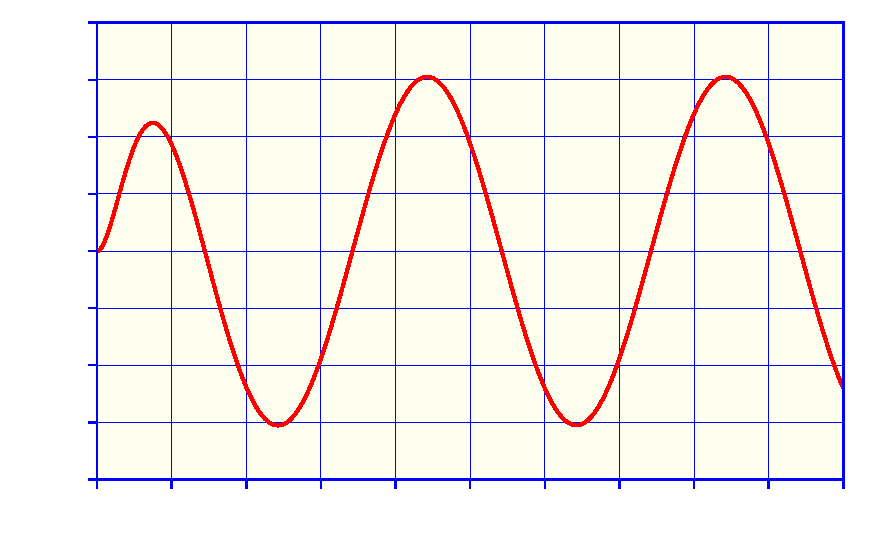
\includegraphics{Cap-Laplace-Exemple4-Tensio}}%
    \gplfronttext
  \end{picture}%
\endgroup

    \end{center}

    La part més feixuga de la resolució d'aquest exemple és l'obtenció de les fraccions parcials, i la posterior obtenció de l'equació temporal utilitzant la taula \ref{taula:Trans-Laplace-Fun}. Aquesta resolució resulta força més fàcil utilitzant la calculadora \emph{HP Prime};
    \index{HP Prime!exemples}els passos a seguir són els següents:

    \begin{dingautolist}{'312}

        \item Per començar premem la tecla 
\includegraphics{HPPrime-CAS.pdf} «computer algebra system», per tal de posar la calculadora en el mode de resolució simbòlic; a continuació premem la tecla 
\includegraphics{HPPrime-Tool.pdf} i escollim \funsfbs{Inverse Laplace} (funció \funsfbs{ilaplace}).

            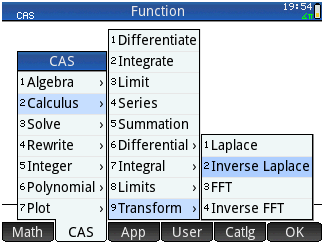
\includegraphics{Cap-Laplace-HPP1.png}

         \item Tot seguit entrem el tres paràmetres que requereix la funció \funsfbs{ilaplace}; el primer és la transformada de Laplace  $U\ped{C}(s)$, el segon és la variable $s$ utilitzada en aquesta expressió, i el tercer és la variable $t$ que volem que aparegui en la transformada inversa de Laplace que ens donarà aquesta funció com a resultat. Quan la calculadora treballa en el  mode de resolució simbòlic cal utilitzar lletres minúscules pels noms de les variables.

            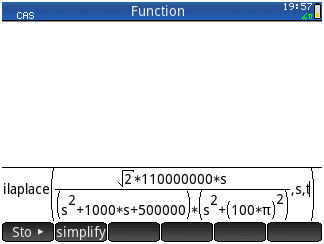
\includegraphics{Cap-Laplace-HPP2.png}\vspace{5mm}

         \item Premem ara la tecla 
\includegraphics{HPPrime-Enter.pdf} i la calculadora ens dona la solució. L'expressió és força llarga, i per veure'n les parts ocultes només cal marcar-la amb el dit i desplaçar-la horitzontalment.

            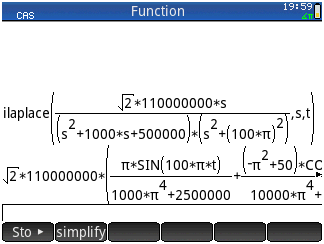
\includegraphics{Cap-Laplace-HPP3.png}\vspace{5mm}

         \item Per  poder representar la gràfica d'aquesta funció, hem d'assignar l'expressió trobada a la  funció \funsfbs{F1}, alhora que canviem la variable \funsfbs{t} per la variable \funsfbs{X}. El primer pas consisteix en marcar amb el dit l'expressió obtinguda anteriorment.

            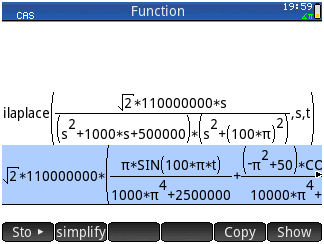
\includegraphics{Cap-Laplace-HPP4.png}\vspace{5mm}

         \item A continuació premem el botó  \hpbutton{Copy}, premem el botó \hpbutton{Sto\hspace{1mm}\faCaretRight} i  escrivim  \funsfbs{F1(t)}.

             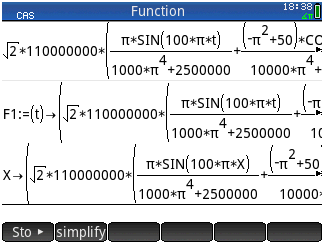
\includegraphics{Cap-Laplace-HPP5.png}\vspace{5mm}

         \item Finalment premem la tecla 
\includegraphics{HPPrime-Enter.pdf}. La variable \funsfbs{t} queda substituïda per la variable \funsfbs{X} i es crea la funció \funsfbs{F1(X)}.

          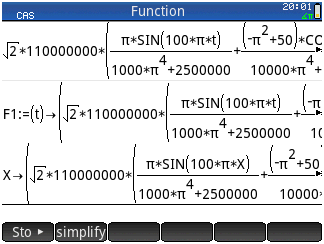
\includegraphics{Cap-Laplace-HPP6.png}\vspace{5mm}


         \item A continuació premem  la tecla 
\includegraphics{HPPrime-Apps.pdf} i seleccionem  l'aplicació \funsfbs{Function}.

            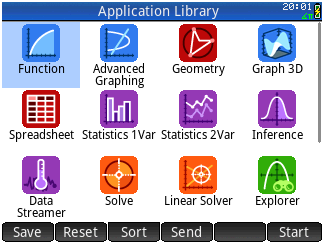
\includegraphics{Cap-Laplace-HPP7.png}\vspace{5mm}

          \item El camp  \funsfbs{F1(X)}, com es pot veure, ja conté l'expressió que volem representar amb  \funsfbs{X} com a variable, gràcies a les operacions fetes en els passos 4 a 6. La \funsfbs{X} majúscula és l'únic nom de variable que accepta aquesta aplicació.

            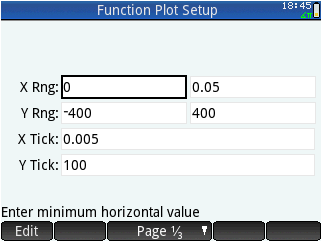
\includegraphics{Cap-Laplace-HPP8.png}\vspace{5mm}

          \item Ara ja podem dibuixar aquesta funció. Comencem ajustant els paràmetres de la gràfica prement les tecles 
\includegraphics{HPPrime-Shift.pdf} 
\includegraphics{HPPrime-Plot.pdf}; fixem els dos valors de \funsfbs{X Rng} a \funsfbs{0} i \funsfbs{0.05} respectivament, els dos valors de \funsfbs{Y Rng} a \funsfbs{-400} i \funsfbs{400} respectivament, el valor de \funsfbs{X Tick} a \funsfbs{0.005}, i el valor de \funsfbs{Y Tick} a \funsfbs{100}.

            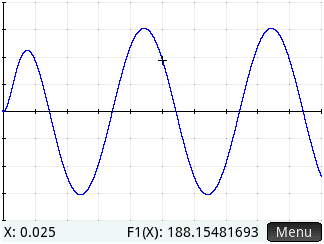
\includegraphics{Cap-Laplace-HPP9.png}\vspace{5mm}

          \item Finalment premem la tecla 
\includegraphics{HPPrime-Plot.pdf} i la calculadora ens mostra la gràfica de la funció. Cal verificar prèviament que la calculadora estigui en el mode angular radiants, ja que en cas contrari el dibuix que obtindríem no seria correcte.

            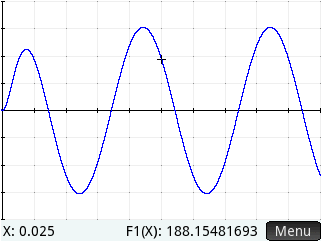
\includegraphics{Cap-Laplace-HPP10.png}

    \end{dingautolist}

\end{exemple}
